\documentclass[../ai_in_finance]{subfiles}
\usepackage[margin=1in]{geometry}
\usepackage{tikz}
\usetikzlibrary{positioning}
\usepackage{amsmath}
\usepackage{amssymb}
\usepackage{booktabs}
\usepackage{draftwatermark}

\SetWatermarkText{Wulin.Suo@Queensu.ca}
\SetWatermarkScale{1.4}
\SetWatermarkColor{gray!35}
\SetWatermarkAngle{45}

\usepackage{makeidx}
\makeindex

\begin{document}

\chapter{Reinforcement Learning in Finance}

\section{Introduction}

Every model built so far in this book, however sophisticated, has answered a single question once. Chapter 6's classifiers predict a label from a feature vector; Chapter 9's credit models predict a default probability; Chapter 11's Almgren-Chriss\index{Almgren-Chriss Model} trajectory prescribes an entire trading schedule, but it does so by solving one optimization problem in advance and then executing the resulting plan. None of these approaches change their answer in response to how the world actually responds to the decisions already made. A portfolio manager, a market maker, and a trading desk do not operate this way: they observe an outcome, update their beliefs, and choose their next action accordingly, over and over, for as long as the position stays open. Reinforcement learning\index{Reinforcement Learning} is the branch of machine learning built specifically for this setting, sequential decision-making under uncertainty, where an agent's own actions influence the future states it will face, and where the right action today depends on the consequences it sets up for tomorrow, not only on today's immediate reward.

This chapter formalizes that setting, the Markov decision process\index{Markov Decision Process (MDP)}, and develops the two families of algorithms built to solve it: value-based methods, culminating in Q-learning\index{Q-Learning} and its neural-network extension, and policy-based methods, culminating in the policy-gradient\index{Policy Gradient} algorithms that power most modern applications. Rather than introducing these ideas in the abstract and only later connecting them to finance, this chapter builds directly on machinery this book has already developed: Chapter 5's binomial-tree early-exercise decision, Chapter 10's portfolio rebalancing problem, and Chapter 11's optimal-execution and market-making models are all, on inspection, special cases of the general sequential-decision problem this chapter formalizes, ones simple enough that a closed-form or backward-induction solution exists. Reinforcement learning is what a practitioner reaches for once the problem is still sequential but no longer simple enough for a closed form, a genuinely common situation once market impact, transaction costs, and a client's actual risk preferences no longer fit the clean functional forms those earlier chapters assumed. The chapter's central worked example makes this connection concrete rather than asserting it: it reframes Chapter 5's American put early-exercise decision as a three-state Markov decision process, solves it with model-free Q-learning instead of backward induction, and shows the learned answer converges to the same value the tree already established, a small, fully verifiable proof that reinforcement learning recovers a known-correct answer before this chapter asks the reader to trust it on problems that have no closed form at all.

The chapter proceeds in three stages. Sections~\ref{sec:rl-framework} through~\ref{sec:rl-taxonomy} build the general Markov decision process framework, the Bellman equation, and the vocabulary, model-based versus model-free, on-policy versus off-policy, needed to place every algorithm that follows. Sections~\ref{sec:rl-qlearning} through~\ref{sec:policy-gradient} develop the algorithms themselves, starting with the fully verifiable tabular Q-learning worked example and building up to deep Q-networks and policy-gradient methods for problems too large for a table. The remaining sections turn to application and honest assessment: optimal execution, market making, and portfolio management (Sections~\ref{sec:rl-execution} through~\ref{sec:rl-multiagent}), a real industry case study (Section~\ref{sec:loxm}), and the evaluation methodology and risks (Sections~\ref{sec:rl-evaluation} and~\ref{sec:rl-challenges}) that separate a reinforcement-learning system that is merely impressive in a backtest from one that is actually safe to deploy with real capital.

\section{The Reinforcement Learning Framework: States, Actions, Rewards, and Policies}\index{Reinforcement Learning Framework}
\label{sec:rl-framework}

A reinforcement learning problem is formalized as a Markov decision process, a tuple $(\mathcal{S}, \mathcal{A}, P, R, \gamma)$. At each discrete time step $t$, an \textbf{agent} observes a \textbf{state} $s_t \in \mathcal{S}$, a summary of everything about the environment relevant to the decision at hand (a market maker's current inventory and the prevailing bid-ask spread; a trading agent's remaining order size and elapsed time; a portfolio manager's current holdings and estimated risk factors). The agent selects an \textbf{action} $a_t \in \mathcal{A}$ (post a quote at a given skew; sell a given number of shares this period; rebalance toward a given target weight) according to a \textbf{policy} $\pi(a \mid s)$, a mapping, possibly stochastic, from states to actions. The environment then transitions to a new state $s_{t+1}$ according to a transition function $P(s_{t+1} \mid s_t, a_t)$ and returns a scalar \textbf{reward} $r_{t+1}$ (realized profit and loss net of costs; a small quadratic risk penalty; an exercise payoff), governed by a reward function $R(s_t, a_t, s_{t+1})$. Figure~\ref{fig:rl_loop} depicts this loop; it repeats until the episode ends, either at a fixed horizon (the market closes, the order is fully executed) or when the agent reaches an absorbing state (a position is liquidated, an option is exercised).

\begin{figure}[htbp]
    \centering
    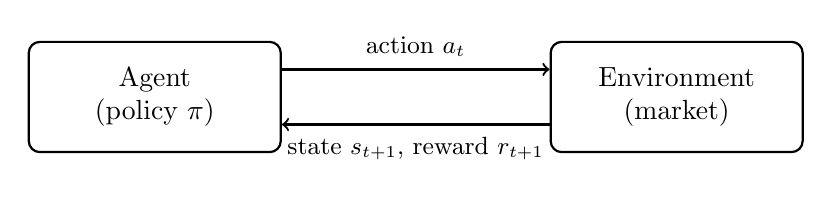
\begin{tikzpicture}[thick,node distance=3.4cm]
        \node[draw,rounded corners,minimum width=3.2cm,minimum height=1.4cm,align=center] (agent) {Agent\\(policy $\pi$)};
        \node[draw,rounded corners,minimum width=3.2cm,minimum height=1.4cm,align=center,right=of agent] (env) {Environment\\(market)};
        \draw[->] ([yshift=0.35cm]agent.east) -- node[above,font=\small,yshift=1pt]{action $a_t$} ([yshift=0.35cm]env.west);
        \draw[->] ([yshift=-0.35cm]env.west) -- node[below,font=\small,yshift=-1pt]{state $s_{t+1}$, reward $r_{t+1}$} ([yshift=-0.35cm]agent.east);
    \end{tikzpicture}
    \caption{The reinforcement learning loop. The agent observes a state and chooses an action according to its policy; the environment responds with a new state and a reward, and the cycle repeats for the length of the episode.}
    \label{fig:rl_loop}
\end{figure}

The word ``Markov'' in Markov decision process is a precise mathematical assumption, not a figure of speech: it requires that $P(s_{t+1} \mid s_t, a_t)$ and $R(s_t, a_t, s_{t+1})$ depend only on the current state and action, not on the full history that led there. This is exactly the assumption behind every stochastic process this book has already used to model prices, from the binomial tree's independent up-and-down moves in Chapter 5 to the random-walk and GARCH innovations of Chapter 7, so it is not a new leap of faith for a reader of this book, only a new name for a familiar structural assumption, now applied to an agent's decisions rather than only to prices themselves. In practice, whether a proposed state representation is genuinely Markovian is itself a design choice: a market maker's state that includes only the current mid-price, and not recent order flow, discards information a real market maker would use, which is why Chapter 12's order-flow-imbalance regression and Chapter 11's Kyle's-lambda\index{Kyle Model: A Formal Model of Price Impact} framework are natural sources of state features for a genuinely useful trading agent, not merely of standalone predictive signals.

The agent's goal is to choose a policy that maximizes the expected \textbf{return}, the discounted sum of future rewards,
\begin{equation*}
G_t = r_{t+1} + \gamma r_{t+2} + \gamma^2 r_{t+3} + \cdots = \sum_{k=0}^{\infty} \gamma^k r_{t+k+1},
\end{equation*}
where the \textbf{discount factor} $\gamma \in [0,1]$ plays a role directly analogous to the discount factor $1/(1+r)$ used everywhere in Chapter 5's valuation formulas: a reward received later is worth less today, both because of the time value of money and, in the reinforcement learning setting, because a reward far in the future is a noisier, harder-to-credit consequence of the current action. A myopic agent with $\gamma = 0$ maximizes only the immediate reward, exactly the one-shot optimization every earlier chapter's models perform; the closer $\gamma$ is to $1$, the more the agent's current choice is shaped by consequences many steps away, which is precisely the additional structure a sequential problem like optimal execution or ongoing portfolio management requires and a one-shot model cannot represent.

\section{From One-Shot Optimization to Sequential Decisions}\index{From One-Shot Optimization to Sequential Decisions}
\label{sec:rl-bridge}

It is worth being explicit about why the models developed in Chapters 10 and 11 did not need this machinery, since the answer clarifies exactly what reinforcement learning adds. The Almgren-Chriss optimal-execution model (Chapter 11's Section 11.8) assumes a known, fixed functional form for market impact, quadratic in the trade rate, and a known, fixed risk-aversion parameter $\lambda$; given those assumptions, the entire optimal trajectory can be solved in closed form in one step, with no need to learn anything from experience, because the model already specifies exactly how the environment will respond to every possible action. Chapter 11's Avellaneda-Stoikov\index{Avellaneda-Stoikov model} inventory model (Section 11.9) is more genuinely dynamic, the market maker's quotes are recomputed at every instant as inventory and time-to-close evolve, but the update rule is itself a closed-form formula derived from an assumed order-arrival process, not a policy learned from trial and error. Chapter 10's Section 10.10 practical-allocation discussion goes furthest toward acknowledging the sequential nature of real portfolio management, noting that rebalancing decisions recur over time and that transaction costs make each rebalancing decision depend on the portfolio's current position, not only on today's estimated optimal weights, but it stops short of solving that sequential problem directly, instead treating each rebalancing decision as a separate, myopic optimization.

Each of these models is exactly right within its assumptions, and each remains the correct tool to reach for whenever those assumptions hold: a known, well-estimated impact function and a well-specified risk-aversion parameter make a closed-form solution both more accurate and vastly cheaper to compute than a learned one. Reinforcement learning becomes the more appropriate tool precisely when that closed form is unavailable, because the true market-impact function is not well approximated by any simple parametric form, because transaction costs interact with the portfolio's history in ways too complex to solve analytically, or because the reward the agent actually cares about, a client's realized utility net of taxes, fees, and behavioral tolerance for drawdowns, does not reduce cleanly to a quadratic cost function at all. In every one of these harder cases, the underlying problem is still a sequential decision problem exactly as formalized in Section~\ref{sec:rl-framework}; what changes is only that no one can write down $P$ and $R$ in closed form, which rules out the direct optimization Chapters 10 and 11 rely on and motivates learning a good policy from simulated or historical experience instead.

\section{Value Functions and the Bellman Equation}\index{Value Functions and the Bellman Equation}
\label{sec:bellman}

Two functions summarize how good a given state, or state-action pair, is under a policy $\pi$: the \textbf{state-value function} $V^\pi(s) = \mathbb{E}_\pi[G_t \mid s_t = s]$, the expected return starting from state $s$ and following $\pi$ thereafter, and the \textbf{action-value function} $Q^\pi(s,a) = \mathbb{E}_\pi[G_t \mid s_t = s, a_t = a]$, the expected return from taking action $a$ in state $s$ and following $\pi$ afterward. Because the return decomposes into an immediate reward plus a discounted continuation, both functions satisfy a recursive relationship, the \textbf{Bellman equation}\index{Bellman Equation}, named for Richard Bellman's original work on dynamic programming:
\begin{equation*}
V^\pi(s) = \sum_a \pi(a \mid s) \sum_{s'} P(s' \mid s, a)\Big[R(s,a,s') + \gamma V^\pi(s')\Big].
\end{equation*}
The \textbf{Bellman optimality equation} specializes this to the best possible policy, replacing the expectation over actions with a maximization:
\begin{equation*}
Q^*(s,a) = \sum_{s'} P(s' \mid s, a)\Big[R(s,a,s') + \gamma \max_{a'} Q^*(s',a')\Big].
\end{equation*}
A reader who worked through Chapter 5's two-step binomial tree (Section 5.9) has already solved a Bellman optimality equation by hand without that name attached to it: at each node, the tree's backward-induction step compares the value of exercising immediately against the discounted expected value of continuing, and takes whichever is larger, exactly the $\max_{a'}$ in the equation above applied to the two actions ``exercise'' and ``hold.'' This is not a loose analogy; Section~\ref{sec:rl-qlearning} makes the correspondence exact by reformulating that identical tree as a Markov decision process and re-deriving the same option value from it. Dynamic programming methods, value iteration and policy iteration, solve the Bellman equation directly whenever $P$ and $R$ are fully known, exactly as Chapter 5's tree does; reinforcement learning's model-free methods, developed next, instead estimate $Q^*$ purely from sampled transitions and rewards, without ever needing $P$ and $R$ written down explicitly, which is the property that makes them applicable to problems, like most real trading and portfolio problems, where no one can specify $P$ and $R$ in closed form to begin with.

\section{A Taxonomy of Reinforcement Learning Methods}\index{Taxonomy of Reinforcement Learning Methods}
\label{sec:rl-taxonomy}

Two further distinctions organize the wide range of reinforcement learning algorithms in use today, and fixing both precisely now makes it easier to place every method the rest of this chapter introduces. Figure~\ref{fig:rl_method_map} previews where each of them fits before the text below explains why.

\begin{figure}[htbp]
    \centering
    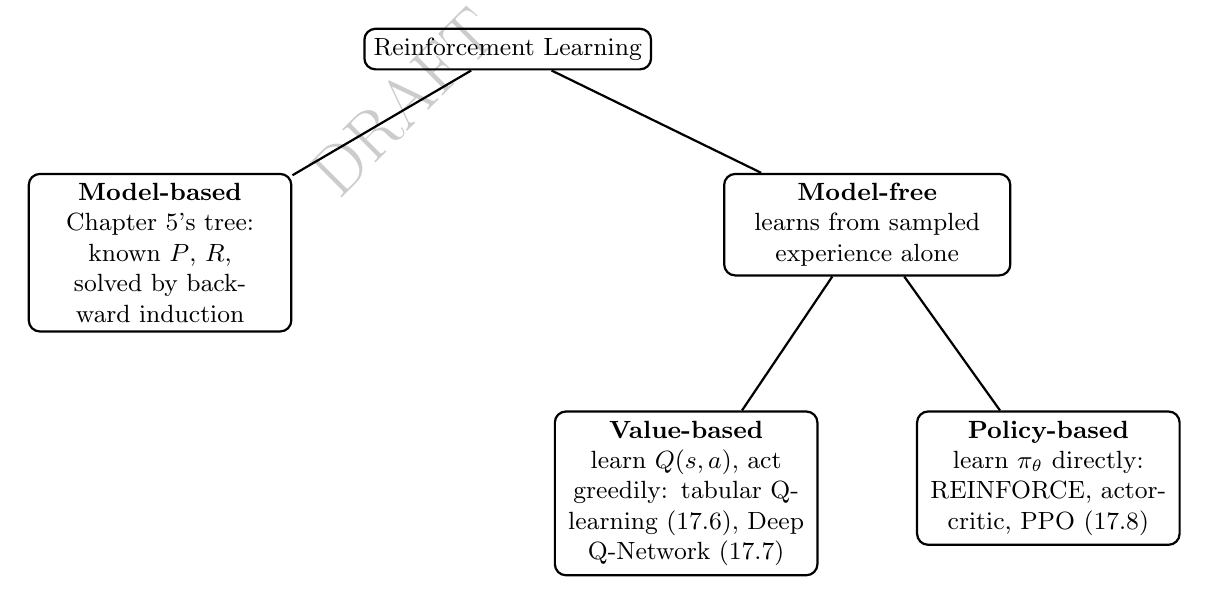
\begin{tikzpicture}[thick,every node/.style={draw,rounded corners,align=center,font=\small},node distance=1.3cm and 0.9cm]
        \node (root) {Reinforcement Learning};
        \node[below left=of root,text width=3.1cm] (mb) {\textbf{Model-based}\\Chapter 5's tree: known $P$, $R$, solved by backward induction};
        \node[below right=of root,text width=3.4cm] (mf) {\textbf{Model-free}\\learns from sampled experience alone};
        \node[below=1.7cm of mf,xshift=-2.3cm,text width=3.1cm] (vb) {\textbf{Value-based}\\learn $Q(s,a)$, act greedily: tabular Q-learning (17.6), Deep Q-Network (17.7)};
        \node[below=1.7cm of mf,xshift=2.3cm,text width=3.1cm] (pb) {\textbf{Policy-based}\\learn $\pi_\theta$ directly: REINFORCE, actor-critic, PPO (17.8)};
        \draw (root) -- (mb);
        \draw (root) -- (mf);
        \draw (mf) -- (vb);
        \draw (mf) -- (pb);
    \end{tikzpicture}
    \caption{A map of the reinforcement learning methods this chapter develops. The model-based/model-free split and the value-based/policy-based split within model-free methods are explained below; Table~\ref{tab:rl_methods} compares the four leaf methods in more detail.}
    \label{fig:rl_method_map}
\end{figure}

\textbf{Model-based methods} have access to, or explicitly learn, the transition function $P$ and reward function $R$ themselves, and use them to plan. Chapter 5's binomial tree is a model-based method: $q$, $u$, $d$, and every terminal payoff are known in advance, so backward induction can compute the exact optimal value with no simulated experience required at all.

\textbf{Model-free methods} never estimate $P$ or $R$ directly; they learn a value function or a policy purely from sampled transitions and rewards, treating the environment as a black box that can be queried (by simulating an episode) but not inspected. Every method developed in the remainder of this chapter, tabular Q-learning, deep Q-networks, and the policy-gradient family, is model-free, which is precisely why each remains usable in the realistic settings Section~\ref{sec:rl-bridge} described, where no closed-form $P$ and $R$ exist for a real limit order book or a real client's multi-period utility.

A third, hybrid category, sometimes called \textbf{learned-model-based methods}, trains an approximate model of $P$ and $R$ directly from data (rather than assuming it, as Chapter 5's tree does) and then plans against that learned model, gaining some of model-based planning's sample efficiency without requiring the transition and reward functions to be known in closed form in advance. This hybrid approach underlies some of reinforcement learning's most prominent successes outside finance, including the game-playing systems that combine a learned model with tree search, but it introduces its own risk, exactly the sim-to-real gap Section~\ref{sec:rl-evaluation} discusses, since a plan is only as good as the learned model it is built against.

\textbf{Off-policy methods} learn about a policy different from the one actually generating their training data. Q-learning's update rule is a clear example: its bootstrapped target uses $\max_{a'} Q(s',a')$, the value of the best available action, regardless of which action the $\varepsilon$-greedy behavior policy actually selected next. This lets a single stream of exploratory, partly random experience be reused to learn about the greedy-optimal policy even while the agent is still busy exploring, exactly why Section~\ref{sec:rl-qlearning}'s worked example converges to the correct answer despite spending a meaningful fraction of its $100{,}000$ episodes taking deliberately random actions. Off-policy methods have a clear data-efficiency advantage, one batch of experience can be reused across many rounds of learning, exactly why DQN's replay buffer (Section~\ref{sec:dqn}) works at all.

\textbf{On-policy methods} instead evaluate and improve exactly the policy currently being followed. The classic on-policy analogue of Q-learning, SARSA\index{SARSA} (State-Action-Reward-State-Action), differs only by replacing $\max_{a'} Q(s',a')$ with $Q(s',a')$ for the action $a'$ the policy actually selects next, so its learned values reflect the actual, still-exploring policy's behavior rather than the ultimate greedy target. Policy-gradient methods (Section~\ref{sec:policy-gradient}) are typically on-policy as well, since their gradient estimator is only valid for returns actually experienced under the current policy $\pi_\theta$, not under some other, older policy. On-policy methods are generally simpler to reason about and more stable to train than off-policy methods, since they never have to correct for a mismatch between the policy that generated the data and the policy currently being evaluated.

\section{A Worked Example: Q-Learning Recovers Chapter 5's Early-Exercise Decision}\index{Q-Learning Recovers Chapter 5's Early-Exercise Decision}
\label{sec:rl-qlearning}

\subsection{Setting Up the Markov Decision Process}

Chapter 5's American put example used a two-step binomial tree with $S_0 = K = \$50$, up and down factors $u=1.2$ and $d=0.9$, and a gross risk-free return $R=1.04$ per period, giving a risk-neutral up-probability $q = (R-d)/(u-d) = 0.14/0.30 \approx 0.4667$ and a per-step discount factor $\gamma = 1/R \approx 0.9615$.

That tree has exactly three decision points: today, at $S_0=\$50$; after one up move, at $S_u=\$60$; and after one down move, at $S_d=\$45$. At each of these three states the holder chooses between two actions: \textbf{exercise}, receive the intrinsic value $\max(K-S,0)$ immediately and end the episode, or \textbf{hold}, receive nothing now and let the tree evolve one more step.

The two terminal nodes reachable only through the up state, $S_{uu}=\$72$ and $S_{ud}=\$54$, both pay $\max(50-S,0)=\$0$; the one terminal node reachable through the down state, $S_{dd}=\$40.50$, pays $\max(50-40.50,0)=\$9.50$.

Putting these pieces together, this is precisely a Markov decision process with states $\mathcal{S}=\{S_0, S_u, S_d\}$ and actions $\mathcal{A}=\{\text{exercise}, \text{hold}\}$, where transition probabilities are given by $q$ and $1-q$, rewards are given by the intrinsic-value and terminal-payoff structure above, and $\gamma=1/R$ discounts every step exactly as Chapter 5's tree already did.

Figure~\ref{fig:mdp_tree} redraws Chapter 5's tree in this chapter's language, labeling each decision node with its two available actions rather than with a single option value.

\begin{figure}[htbp]
    \centering
    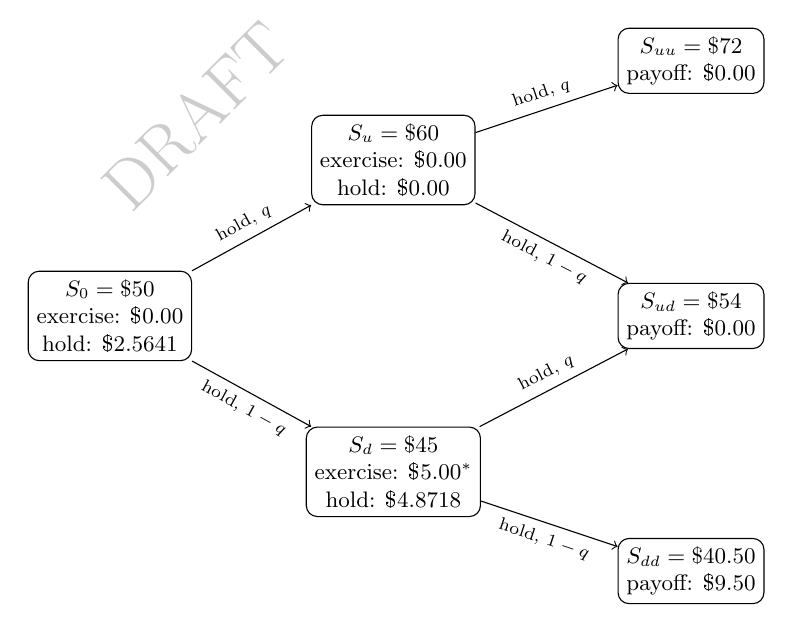
\begin{tikzpicture}[scale=0.9,transform shape,every node/.style={font=\small}]
        \node[draw,rounded corners,align=center] (s0) at (0,0) {$S_0=\$50$\\exercise: \$0.00\\hold: \$2.5641};
        \node[draw,rounded corners,align=center] (su) at (4.0,2.2) {$S_u=\$60$\\exercise: \$0.00\\hold: \$0.00};
        \node[draw,rounded corners,align=center] (sd) at (4.0,-2.2) {$S_d=\$45$\\exercise: \$5.00$^*$\\hold: \$4.8718};
        \node[draw,rounded corners,align=center] (suu) at (8.2,3.6) {$S_{uu}=\$72$\\payoff: \$0.00};
        \node[draw,rounded corners,align=center] (sud) at (8.2,0) {$S_{ud}=\$54$\\payoff: \$0.00};
        \node[draw,rounded corners,align=center] (sdd) at (8.2,-3.6) {$S_{dd}=\$40.50$\\payoff: \$9.50};
        \draw[->] (s0) -- node[above,sloped,font=\scriptsize] {hold, $q$} (su);
        \draw[->] (s0) -- node[below,sloped,font=\scriptsize] {hold, $1-q$} (sd);
        \draw[->] (su) -- node[above,sloped,font=\scriptsize] {hold, $q$} (suu);
        \draw[->] (su) -- node[below,sloped,font=\scriptsize] {hold, $1-q$} (sud);
        \draw[->] (sd) -- node[above,sloped,font=\scriptsize] {hold, $q$} (sud);
        \draw[->] (sd) -- node[below,sloped,font=\scriptsize] {hold, $1-q$} (sdd);
    \end{tikzpicture}
    \caption{The early-exercise decision of Chapter 5's American put, redrawn as a three-state Markov decision process. Each of $S_0$, $S_u$, and $S_d$ lists the closed-form $Q$-value of both available actions, exercise and hold; the down node's exercise value, marked with an asterisk, exceeds its hold value, making exercise the optimal action there and the source of the tree's early-exercise premium. Terminal nodes show the American put's payoff, reached only if the holder chooses hold at every earlier decision point.}
    \label{fig:mdp_tree}
\end{figure}

Chapter 5 solved this exact problem by backward induction, working from the known terminal payoffs back to today. Restated in this chapter's notation, that solution is
\begin{align*}
Q^*(S_u, \text{exercise}) &= \$0.00, & Q^*(S_u, \text{hold}) &= \gamma\big[q(0) + (1-q)(0)\big] = \$0.00,\\
Q^*(S_d, \text{exercise}) &= \$5.00, & Q^*(S_d, \text{hold}) &= \gamma\big[q(0) + (1-q)(9.50)\big] \approx \$4.8718,\\
Q^*(S_0, \text{exercise}) &= \$0.00, & Q^*(S_0, \text{hold}) &= \gamma\big[q\,V^*(S_u) + (1-q)\,V^*(S_d)\big] \approx \$2.5641,
\end{align*}
where $V^*(S_u)=\max(0.00,0.00)=\$0.00$ and $V^*(S_d)=\max(5.00,4.8718)=\$5.00$, since exercising is optimal at the down node. The optimal policy is therefore to hold at $S_0$ and $S_u$ and exercise at $S_d$, giving an American put value of $V^*(S_0) \approx \$2.5641$, exactly the value Chapter 5 reports.

\subsection{Tabular Q-Learning}

Backward induction requires knowing $q$, $\gamma$, and every terminal payoff in advance, exactly the closed-form knowledge Section~\ref{sec:rl-bridge} argued is unavailable in most real trading and portfolio problems. \textbf{Q-learning} instead estimates $Q^*$ from simulated experience alone, never using $q$ directly in its update rule. Starting from an arbitrary initial table $Q(s,a)$ (here, all zeros), the agent repeatedly simulates an episode: at each state it chooses an action using an $\varepsilon$-greedy policy (with probability $\varepsilon$, act randomly to keep exploring; otherwise, act greedily with respect to the current $Q$-table), observes the resulting reward $r$ and next state $s'$, and updates
\begin{equation*}
Q(s,a) \leftarrow Q(s,a) + \alpha\Big[r + \gamma \max_{a'} Q(s',a') - Q(s,a)\Big],
\end{equation*}
where $\alpha$ is a learning rate. This update rule, known as \textbf{temporal-difference learning}\index{Temporal-Difference Learning}, nudges the current estimate $Q(s,a)$ toward a bootstrapped target, the observed reward plus the discounted value of the best action available in the next state, without ever requiring a model of the transition probabilities; the agent learns $q$'s effect on the optimal decision purely by observing many simulated up and down moves and seeing which actions paid off, in exactly the same statistical spirit as every other machine learning method in this book learning a relationship from data rather than being told it directly.

The companion notebook simulates this process for $100{,}000$ episodes, using a learning rate that decays with each state-action pair's visit count and an exploration rate $\varepsilon$ that decays from $0.30$ to $0.02$ over training, standard choices that guarantee enough early exploration to discover the exercise decision at $S_d$ while still converging to a stable, greedy policy by the end of training. Table~\ref{tab:rl_qlearning} compares the learned $Q$-table to the closed-form values derived above.

\begin{table}[htbp]
\centering
\caption{Closed-form Bellman-optimal $Q$-values (from backward induction) versus tabular Q-learning's learned estimates after 100,000 simulated episodes.}
\label{tab:rl_qlearning}
\begin{tabular}{lccc}
\toprule
State-action & Closed-form $Q^*$ & Learned $Q$ (Q-learning) & Relative gap \\
\midrule
$(S_0, \text{exercise})$ & \$0.0000 & \$0.0000 & --- \\
$(S_0, \text{hold})$ & \$2.5641 & \$2.5328 & $1.22\%$ \\
$(S_u, \text{exercise})$ & \$0.0000 & \$0.0000 & --- \\
$(S_u, \text{hold})$ & \$0.0000 & \$0.0000 & --- \\
$(S_d, \text{exercise})$ & \$5.0000 & \$5.0000 & $0.00\%$ \\
$(S_d, \text{hold})$ & \$4.8718 & \$4.9234 & $1.06\%$ \\
\bottomrule
\end{tabular}
\end{table}

\subsection{Comparing the Learned and Closed-Form Solutions}

The learned policy matches the closed-form optimal policy exactly: hold at $S_0$ ($\$2.5328 > \$0.0000$), exercise at 
$S_d$ ($\$5.0000 > \$4.9234$), and, at $S_u$, both actions are learned as worth $\$0.0000$, an exact tie that matches Chapter 5's own 
observation that ``both exercise and continuation are worth \$0'' at that node, so which action the tie-break happens to favor is 
economically inconsequential. Every ``exercise'' value converges exactly, with no residual error, since exercising ends the episode 
immediately and its reward is observed without any noise; every ``hold'' value converges to within roughly $1\%$ of the true value but 
not exactly, since a ``hold'' estimate is a bootstrapped average built from a finite number of noisy sampled continuations rather than 
an exact expectation computed from a known $q$. 

This gap is not a bug to be engineered away; it is the fundamental price of model-free 
learning, and it is the single most important lesson this worked example offers: when the transition probabilities and payoffs are 
genuinely known in closed form, as they are in Chapter 5's tree, backward induction is strictly better, exact, instantaneous, 
and requiring no simulated data at all, and reinforcement learning should not be used. Reinforcement learning earns its keep only 
in the more realistic setting, developed throughout the rest of this chapter, where no such closed form exists and simulated or 
historical experience is the only source of information available.

\section{From Tables to Function Approximation: Deep Q-Networks}\index{Deep Q-Network (DQN)}
\label{sec:dqn}

Tabular Q-learning stores one number for every state-action pair, which works only because Section~\ref{sec:rl-qlearning}'s example has just three states and two actions. A realistic trading state, some combination of inventory, elapsed time, recent order-flow imbalance (Chapter 12), and a handful of price-based features, takes values from a continuous or extremely large discrete space, making an explicit table impossible to store or to visit often enough to fill in. The standard fix, introduced by Mnih et al.\ (2015) and known as the \textbf{Deep Q-Network} (DQN), replaces the table with a neural network $Q(s,a;\theta)$, exactly the feedforward architecture Chapter 6's Section 6.18 introduced, trained to approximate the same Bellman-optimal $Q^*$ function. The network takes a state (or a fixed-size feature vector describing one) as input and outputs one value per possible action; training minimizes the squared temporal-difference error,
\begin{equation*}
\mathcal{L}(\theta) = \mathbb{E}\Big[\big(r + \gamma \max_{a'} Q(s',a';\theta^-) - Q(s,a;\theta)\big)^2\Big],
\end{equation*}
using the same gradient-descent machinery Chapter 6's Section 6.5 already developed for supervised learning, with $\theta^-$ a periodically-updated copy of the network's own parameters (a ``target network'') used to keep the bootstrapped target from chasing a constantly-moving estimate, one of two stabilization tricks, alongside storing and randomly resampling past transitions from a large ``replay buffer'' rather than training only on the most recent experience, that made deep Q-learning reliable enough to train at all. The underlying update rule is otherwise identical to tabular Q-learning: the network simply generalizes across similar states instead of memorizing each one independently, letting the agent act sensibly in a state it has never visited before, provided that state resembles ones it has seen, exactly the same generalization argument that justifies every other neural network in this book.

Deep Q-networks are also considerably more finicky to train than tabular Q-learning, in a way worth naming explicitly given this book's repeated warnings, in Chapter 10's badly-scaled optimizer example among others, that a plausible-looking numerical method can silently fail to converge without an obvious error message. A DQN's training loss can decrease steadily while the actual learned policy remains poor, since the loss measures how well the network fits its own, still-inaccurate bootstrapped targets rather than how good the resulting policy actually is; the only reliable check is to evaluate the policy's real performance directly, exactly the discipline Section~\ref{sec:rl-qlearning}'s worked example applied by comparing learned $Q$-values against an independently known closed-form answer, and exactly the discipline Section~\ref{sec:rl-evaluation} generalizes into a full evaluation methodology for problems where no closed-form answer exists to check against.

\section{Policy Gradient Methods and Continuous Actions}\index{Policy Gradient}
\label{sec:policy-gradient}

Q-learning and its deep variant both learn a value function and derive a policy from it implicitly, by acting greedily. This works cleanly when the action set is small and discrete, exercise or hold, buy or sell, but breaks down when the natural action is continuous, exactly how many shares to trade this period, or exactly what target weight to assign an asset, since $\max_{a'} Q(s',a')$ has no simple closed form once $a'$ ranges over a continuum. \textbf{Policy gradient} methods sidestep this by parameterizing the policy directly, $\pi_\theta(a \mid s)$, typically as a neural network outputting the parameters of a continuous distribution (a mean and standard deviation, for instance), and adjusting $\theta$ to directly increase the expected return, using the policy gradient theorem,
\begin{equation*}
\nabla_\theta J(\theta) = \mathbb{E}_{\pi_\theta}\Big[\nabla_\theta \log \pi_\theta(a \mid s) \, G_t\Big],
\end{equation*}
which says, informally, that actions followed by a higher-than-expected return should be made more likely, and actions followed by a lower-than-expected return should be made less likely, with the size of the nudge proportional to how surprising the return was.

\textbf{Actor-critic}\index{Actor-Critic} methods reduce the noise in this estimate by learning a value function (the ``critic'') alongside the policy (the ``actor'') and using it to judge whether a given return was better or worse than expected from that state, rather than judging it against the raw, highly variable return alone.

\textbf{Proximal Policy Optimization}\index{Proximal Policy Optimization (PPO)} (PPO), introduced by Schulman et al.\ (2017), is the most widely used modern policy-gradient algorithm. It constrains each policy update to stay close to the previous policy, preventing the large, destabilizing updates that plagued earlier policy-gradient methods, and its combination of reasonable sample efficiency and training stability has made it the default starting point for continuous-action problems across robotics, game-playing, and, increasingly, the trading and portfolio applications developed next.

Table~\ref{tab:rl_methods} summarizes the four families of methods this chapter has introduced, alongside the setting each is best suited to and the concrete finance application, developed in the sections that follow, each is most naturally applied to.

\begin{table}[htbp]
\centering
\caption{A summary of the reinforcement learning methods introduced in this chapter.}
\label{tab:rl_methods}
\begin{tabular}{p{2.6cm}p{2.3cm}p{2.3cm}p{6.3cm}}
\toprule
Method & Learns & Best suited to & Natural finance application \\
\midrule
Tabular Q-learning & Action-value function $Q(s,a)$ & Small, discrete state and action spaces & Section~\ref{sec:rl-qlearning}'s early-exercise decision; small discretized inventory or execution problems \\
Deep Q-Network (DQN) & Neural-network approximation of $Q(s,a;\theta)$ & Large or continuous state spaces, discrete actions & Execution and market-making agents (Section~\ref{sec:rl-execution}) with rich order-book state features \\
Policy gradient (REINFORCE, actor-critic) & A parameterized policy $\pi_\theta(a\mid s)$ directly & Continuous action spaces & Trade-size or quote-skew decisions that vary continuously rather than over a small discrete menu \\
Proximal Policy Optimization (PPO) & A parameterized policy, with a stabilized update rule & Continuous actions, need for reliable, stable training & Portfolio-rebalancing agents (Section~\ref{sec:rl-portfolio}) and production execution systems such as Section~\ref{sec:loxm}'s LOXM \\
\bottomrule
\end{tabular}
\end{table}

\section{Learning from Expert Demonstrations: Imitation and Inverse Reinforcement Learning}\index{Imitation Learning}
\label{sec:imitation}

Every method developed so far learns purely from trial and error, an agent that starts knowing nothing about which actions are good must discover this for itself through the $\varepsilon$-greedy exploration of Section~\ref{sec:rl-qlearning} or its neural-network analogues. When a record of a skilled human decision-maker's past choices already exists, an experienced trader's execution decisions, say, a faster alternative is available: \textbf{behavioral cloning}\index{Behavioral Cloning} treats the expert's historical state-action pairs as an ordinary supervised training set and fits a policy $\pi_\theta(a\mid s)$ to predict the expert's action from the state, using exactly the same classification machinery Chapter 6 developed, sidestepping reinforcement learning's exploration problem entirely by never requiring the agent to try an action the expert did not.

Behavioral cloning has a well-known weakness: it is only ever as good as the expert it imitates, and it can fail badly in states the expert rarely visited, since a supervised classifier trained only on an expert's typical behavior has no guidance for how to recover once the agent's own small errors push it into an unfamiliar state the expert's demonstrations never covered, compounding over a long trajectory in a way a single supervised prediction never does. \textbf{Inverse reinforcement learning}\index{Inverse Reinforcement Learning} takes a different approach to the same underlying idea: rather than directly imitating the expert's actions, it infers the reward function the expert appears to be optimizing, and then solves the resulting Markov decision process using this chapter's own methods, producing a policy that can, in principle, generalize sensibly to states the expert never actually visited, at the cost of a harder and less well-posed estimation problem, since many different reward functions can often rationalize the same observed expert behavior equally well.

Both techniques are directly relevant to the applications developed next: a system like Section~\ref{sec:loxm}'s LOXM, reported to be trained on ``a large history of past trades together with simulated trading scenarios,'' plausibly combines exactly this kind of demonstration-based learning, bootstrapping an initial policy from historical human and algorithmic execution decisions, with further trial-and-error refinement in simulation, rather than learning a trading policy from pure, unguided exploration alone. This hybrid approach is common in practice precisely because it addresses reinforcement learning's sample-inefficiency problem directly: starting from a reasonable, expert-informed policy rather than from nothing gives the trial-and-error refinement stage a far smaller gap to close, exactly the practical advantage that makes imitation-based pretraining worth the additional complexity in a genuinely high-stakes application.

\section{Reinforcement Learning for Optimal Execution and Market Making}\index{Reinforcement Learning for Optimal Execution and Market Making}
\label{sec:rl-execution}

Optimal execution was among the earliest documented applications of reinforcement learning in finance: Nevmyvaka, Feng, and Kearns (2006) applied tabular Q-learning, structurally similar to Section~\ref{sec:rl-qlearning}'s worked example but with a far larger state space built from order-book features, to real historical limit order book data and found that a learned execution policy could meaningfully reduce trading costs relative to the simple TWAP and VWAP\index{TWAP and VWAP: Basic Execution Algorithms} benchmarks Chapter 11's Section 11.7 introduced, without ever being given a closed-form market-impact model to optimize against. The state in a modern version of this problem typically includes remaining inventory, time remaining in the execution window, the current bid-ask spread, and recent order-flow imbalance; the action is how many shares to submit, and at what limit price, this period; and the reward is the negative implementation shortfall (Chapter 11's Section 11.14 transaction-cost-analysis measure) realized on that period's fill. Unlike Almgren-Chriss, which commits in advance to a fixed schedule regardless of how the market subsequently behaves, a reinforcement-learned execution policy can condition its trade size on the order book it actually observes, trading faster when liquidity is unusually deep and slowing down when the book thins out, a genuinely adaptive behavior no closed-form schedule can replicate.

\subsection{A Worked Example: Q-Learning Recovers the Almgren-Chriss Optimal Trajectory}\index{Q-Learning Recovers the Almgren-Chriss Optimal Trajectory}
\label{sec:rl-execution-worked}

Section~\ref{sec:rl-qlearning}'s worked example verified Q-learning against a known answer on a small, three-state problem. It is worth doing the same on a problem closer to genuine trading practice: Chapter 11's own Almgren-Chriss worked example, the $250$-share order split across $N=5$ intervals with impact coefficient $\eta=0.01$, per-interval volatility $\sigma=2\%$, and risk aversion $\lambda=0.5$, whose closed-form optimal trajectory left unexecuted shares $(250,\ 194.2,\ 142.4,\ 93.4,\ 46.2,\ 0)$ at a total risk-adjusted cost of $139.4$.

Reformulated as a Markov decision process, the state at interval $j$ is the inventory $x_{j-1}$ still unexecuted, discretized to the nearest $5$ shares (a grid of $51$ possible inventory levels), and the action is how many of those shares, again in multiples of $5$, to sell this interval. The reward for selling $a_j$ shares and leaving $x_j=x_{j-1}-a_j$ unexecuted is the negative of Chapter 11's own per-interval cost,
\begin{equation*}
r_j = -\left[\eta\,\frac{a_j^2}{\tau} + \lambda\sigma^2\tau\, x_j^2\right],
\end{equation*}
with $\tau=1$ matching Chapter 11's own normalization, and the last interval ($j=5$) forces full liquidation, $x_5=0$, exactly as the closed-form problem requires. Unlike Section~\ref{sec:rl-qlearning}'s tree, this environment is entirely \textbf{deterministic}: choosing an action leaves no residual uncertainty about the resulting state or reward, since Almgren-Chriss prices timing risk analytically through the variance term $\lambda\sigma^2\tau x_j^2$ rather than by exposing the agent to a randomly sampled price path. Reinforcement learning is still the right tool here for a different reason than in Section~\ref{sec:rl-qlearning}: not to cope with stochastic transitions, but to search a state-action space of roughly $5{,}300$ discretized possibilities, far too many to enumerate by hand, without ever being given the closed-form $\sinh(\cdot)$ trajectory formula Chapter 11 derived analytically.

Exact backward-induction dynamic programming over this same discretized grid, computable directly since only $51$ inventory levels and $4$ real decision points are involved, gives an optimal discretized trajectory of $(250,\ 195,\ 145,\ 95,\ 45,\ 0)$ shares at a total cost of $139.52$, close to but not identical to the continuous closed-form values, an expected consequence of rounding a continuous optimum onto a $5$-share grid rather than any error in the discretization itself. Tabular Q-learning, trained model-free for $600{,}000$ episodes with an $\varepsilon$-greedy behavior policy decaying from $\varepsilon=0.5$ to $0.05$ and a visit-count-decayed learning rate, \textbf{converges to exactly this same trajectory and exactly this same cost}, $139.52$, not merely close to it. This is a meaningfully different outcome from Section~\ref{sec:rl-qlearning}'s worked example, where the learned ``hold'' values settled within roughly one percent of their closed-form targets rather than matching them exactly: because this environment is deterministic, every reward Q-learning observes is noise-free, so once training has explored a state-action pair enough times to identify its best continuation, the learned value converges to it exactly, with no residual estimation error left to average away.

Figure~\ref{fig:dp_backward_induction} makes the backward-induction computation itself concrete. Dynamic programming does not work through the five intervals in the order a trader would experience them; it starts from the one stage with no real decision left, the forced liquidation at $x_4$, and solves backward, one stage at a time, using each already-solved stage's value function to solve the one before it, until $V_1(x_0)$ finally gives the answer for the full, five-interval problem. Only after this entire backward pass is complete can the optimal trajectory be traced forward, choosing at each state whichever action attains the value just computed for it, exactly the bottom row of the figure.

\begin{figure}[htbp]
    \centering
    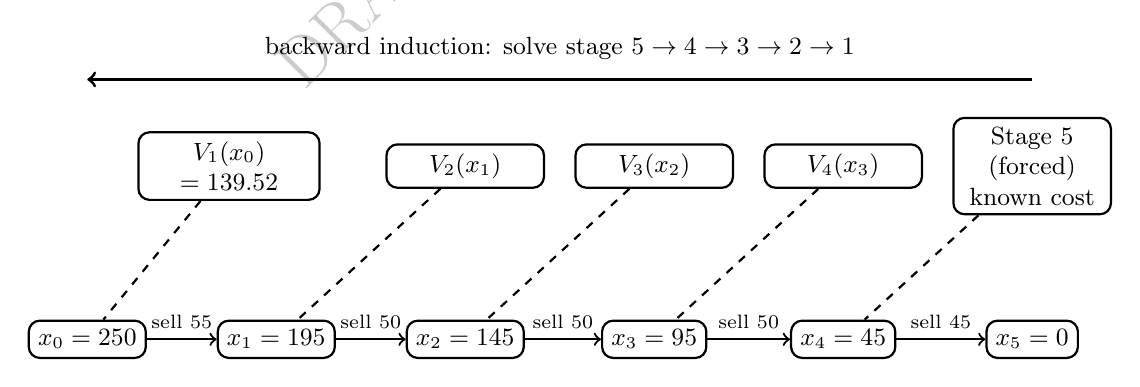
\begin{tikzpicture}[thick,every node/.style={font=\small}]
        \draw[->,line width=1.1pt] (12.0,3.3) -- (0,3.3);
        \node[align=center,font=\small] at (6.0,3.7) {backward induction: solve stage $5 \to 4 \to 3 \to 2 \to 1$};
        \node[draw,rounded corners,align=center,minimum width=2.0cm] (v5) at (12.0,2.2) {Stage 5\\(forced)\\known cost};
        \node[draw,rounded corners,align=center,minimum width=2.0cm] (v4) at (9.6,2.2) {$V_4(x_3)$};
        \node[draw,rounded corners,align=center,minimum width=2.0cm] (v3) at (7.2,2.2) {$V_3(x_2)$};
        \node[draw,rounded corners,align=center,minimum width=2.0cm] (v2) at (4.8,2.2) {$V_2(x_1)$};
        \node[draw,rounded corners,align=center,minimum width=2.3cm] (v1) at (1.8,2.2) {$V_1(x_0)$\\$=139.52$};
        \node[draw,rounded corners,align=center] (n0) at (0,0) {$x_0=250$};
        \node[draw,rounded corners,align=center] (n1) at (2.4,0) {$x_1=195$};
        \node[draw,rounded corners,align=center] (n2) at (4.8,0) {$x_2=145$};
        \node[draw,rounded corners,align=center] (n3) at (7.2,0) {$x_3=95$};
        \node[draw,rounded corners,align=center] (n4) at (9.6,0) {$x_4=45$};
        \node[draw,rounded corners,align=center] (n5) at (12.0,0) {$x_5=0$};
        \draw[->] (n0) -- node[above,font=\scriptsize] {sell 55} (n1);
        \draw[->] (n1) -- node[above,font=\scriptsize] {sell 50} (n2);
        \draw[->] (n2) -- node[above,font=\scriptsize] {sell 50} (n3);
        \draw[->] (n3) -- node[above,font=\scriptsize] {sell 50} (n4);
        \draw[->] (n4) -- node[above,font=\scriptsize] {sell 45} (n5);
        \draw[dashed] (v1) -- (n0);
        \draw[dashed] (v2) -- (n1);
        \draw[dashed] (v3) -- (n2);
        \draw[dashed] (v4) -- (n3);
        \draw[dashed] (v5) -- (n4);
    \end{tikzpicture}
    \caption{Backward-induction dynamic programming for the execution problem. The top row is solved right to left: the forced stage-5 liquidation cost is known immediately, then $V_4$, $V_3$, $V_2$, and finally $V_1(x_0)=139.52$, the total cost of the whole five-interval problem, each computed using the value already found for the stage to its right. Only once every value function is known does the bottom row, the optimal trajectory, get traced left to right by following whichever action attains each state's value.}
    \label{fig:dp_backward_induction}
\end{figure}

Table~\ref{tab:rl_execution_compare} places the Q-learning-recovered trajectory alongside the uniform TWAP schedule and the fully aggressive single-shot execution Chapter 11 also scored, confirming the same efficient-frontier ordering Chapter 11 established analytically now emerges from an agent that was never given the underlying cost formula at all.

\begin{table}[htbp]
\centering
\caption{Total risk-adjusted execution cost under three strategies for the same $250$-share, $N=5$-interval order ($\eta=0.01$, $\sigma=2\%$, $\lambda=0.5$).}
\label{tab:rl_execution_compare}
\begin{tabular}{lcc}
\toprule
Strategy & Unexecuted-share trajectory & Total cost \\
\midrule
Fully aggressive (single shot) & $(250, 0, 0, 0, 0, 0)$ & $625.00$ \\
Uniform TWAP & $(250, 200, 150, 100, 50, 0)$ & $140.00$ \\
Q-learning (learned, discretized) & $(250, 195, 145, 95, 45, 0)$ & $139.52$ \\
\bottomrule
\end{tabular}
\end{table}

Figure~\ref{fig:execution_trajectories} plots the same three trajectories, making the front-loading pattern immediately visible: the fully aggressive strategy liquidates instantly, the uniform TWAP schedule is a straight line, and the Q-learning trajectory sits just above TWAP early on, trading a little faster than uniform while inventory is largest and tapering to match TWAP by the final interval, exactly the mild front-loading Chapter 11's continuous closed-form solution also produced.

\begin{figure}[htbp]
    \centering
    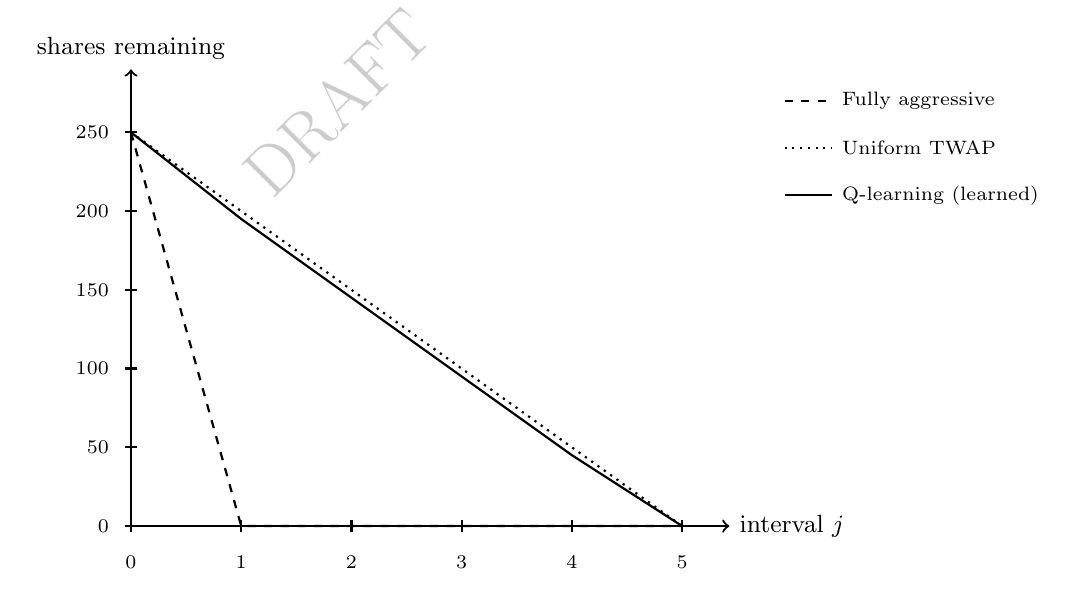
\begin{tikzpicture}[thick]
        \draw[->] (0,0) -- (7.6,0) node[right,font=\small] {interval $j$};
        \draw[->] (0,0) -- (0,5.8) node[above,font=\small] {shares remaining};
        \foreach \i in {0,1,2,3,4,5} {
            \draw (\i*1.4,0.08) -- (\i*1.4,-0.08);
            \node[below,font=\scriptsize] at (\i*1.4,-0.25) {\i};
        }
        \foreach \y/\lab in {0/0,1/50,2/100,3/150,4/200,5/250} {
            \draw (0.08,\y) -- (-0.08,\y);
            \node[left,font=\scriptsize] at (-0.15,\y) {\lab};
        }
        \draw[dashed] plot coordinates {(0,5) (1.4,0) (2.8,0) (4.2,0) (5.6,0) (7.0,0)};
        \draw[dotted] plot coordinates {(0,5) (1.4,4) (2.8,3) (4.2,2) (5.6,1) (7.0,0)};
        \draw[solid] plot coordinates {(0,5) (1.4,3.9) (2.8,2.9) (4.2,1.9) (5.6,0.9) (7.0,0)};
        \draw[dashed] (8.3,5.4) -- (8.9,5.4); \node[right,font=\scriptsize] at (8.9,5.4) {Fully aggressive};
        \draw[dotted] (8.3,4.8) -- (8.9,4.8); \node[right,font=\scriptsize] at (8.9,4.8) {Uniform TWAP};
        \draw[solid] (8.3,4.2) -- (8.9,4.2); \node[right,font=\scriptsize] at (8.9,4.2) {Q-learning (learned)};
    \end{tikzpicture}
    \caption{Unexecuted-share trajectories under the three strategies of Table~\ref{tab:rl_execution_compare}. The learned Q-learning trajectory closely tracks uniform TWAP but trades slightly faster in the first two intervals, the same mild front-loading Chapter 11's closed-form solution derives analytically for a modestly risk-averse trader.}
    \label{fig:execution_trajectories}
\end{figure}

Market making extends naturally to the same framework. Chapter 11's Avellaneda-Stoikov model derives a closed-form optimal quote skew from an assumed order-arrival intensity function and a known risk-aversion parameter; a reinforcement-learning market maker instead learns a quoting policy directly from simulated or historical order flow, with state features again drawn from current inventory, time-to-close, and order-book depth, action given by the bid and ask quotes (or, in a simplified discrete-action version, a small set of candidate skews), and reward given by realized spread capture net of inventory risk and adverse selection, the same adverse-selection concern Chapter 12's Glosten-Milgrom\index{Glosten-Milgrom model} model formalizes. The appeal is identical to the execution case: a learned policy can adapt to order-arrival patterns that deviate from Avellaneda-Stoikov's assumed functional form, at the cost of requiring a large amount of representative training data and offering none of the closed-form model's transparency about why a given quote was chosen, a tradeoff this chapter's closing sections return to directly.

\subsection{Designing States, Actions, and Rewards in Practice}

Neither problem above specifies its Markov decision process uniquely, and the specific design choices a practitioner makes matter enormously to whether the resulting agent actually learns something useful. A state representation that omits recent order-flow imbalance discards exactly the predictive signal Chapter 12's order-flow-imbalance regression showed carries real information about near-term price movement, weakening the agent below what a well-informed human trader, or a simpler rule-based system that explicitly conditions on that signal, could achieve; a state that includes too many redundant or noisy features, conversely, slows learning by forcing the agent to discover on its own which features actually matter, exactly the feature-engineering discipline Chapter 6's Section 6.14 already developed for supervised models, now facing the added difficulty that a reinforcement-learning agent must learn this from its own trial and error rather than from a fixed, already-labeled training set.

Reward design carries the same tension in sharper form, because Section~\ref{sec:rl-challenges} shows that an imperfect reward does not merely produce a slightly worse agent, it produces an agent that is often precisely, confidently wrong about what it is optimizing. A common practical compromise is to shape the reward with an intermediate, densely observed signal, a small penalty proportional to inventory held at each step, say, in addition to the sparse, terminal profit-and-loss outcome, which speeds up learning considerably (the agent gets useful feedback every step rather than only at the end of a long execution episode) but introduces its own risk: if the shaping term is not carefully scaled relative to the true objective, the agent can learn to over-optimize the intermediate proxy (holding needlessly little inventory, say) at the expense of the actual goal it was meant merely to support learning toward. There is no universal recipe for getting this balance right; in practice it is validated the same way any other model choice in this book is validated, by comparing the resulting policy's realized, out-of-sample performance against the closed-form or rule-based benchmark it is meant to improve on, exactly as Section~\ref{sec:rl-evaluation} recommends.

\section{Reinforcement Learning for Portfolio Management}\index{Reinforcement Learning for Portfolio Management}
\label{sec:rl-portfolio}

Chapter 10's mean-variance framework solves a single-period allocation problem: given today's estimated expected returns and covariance matrix, find the weights that optimize a risk-return tradeoff today. Section 10.10's practical-allocation discussion acknowledges that real portfolios are rebalanced repeatedly and that transaction costs make each rebalancing decision depend on the portfolio's current position, but it stops at flagging this complexity rather than solving the resulting multi-period problem directly. Framed as a Markov decision process, the state is the portfolio's current holdings together with estimated risk-factor exposures (Chapter 10's Section 10.7 multi-factor model is a natural source of these features); the action is a new target weight vector, or equivalently the trades needed to reach it; and the reward combines the period's realized return with an explicit penalty for transaction costs and, if desired, for realized volatility or drawdown, letting the agent learn a rebalancing policy that trades off today's allocation quality against the cost of getting there, rather than treating every rebalancing decision as a fresh, myopic optimization the way Chapter 10 does.

This framing is genuinely more general than Chapter 10's static optimization, and that generality is exactly its cost. A reinforcement-learning portfolio agent requires either a large amount of representative historical data or a realistic market simulator to train in, since a poorly specified reward (one that fails to penalize drawdown, say, or that rewards raw return without any risk adjustment) will produce a policy that optimizes exactly the wrong objective with no warning that anything has gone wrong, a version of the ``reward hacking'' problem Section~\ref{sec:rl-challenges} discusses in more depth. In practice, most institutional applications of reinforcement learning to portfolio management remain closer to research than to production, used to explore whether a learned, adaptive rebalancing policy can outperform Chapter 10's static mean-variance benchmark net of realistic transaction costs, rather than to replace that benchmark outright; the honest current state of the field is that reinforcement learning has demonstrated clearer, more reproducible gains in the execution and market-making applications of Section~\ref{sec:rl-execution}, where the reward (realized trading cost) is comparatively unambiguous to specify, than in full portfolio management, where the ``right'' reward is itself a genuinely open question tied to a client's actual, often unstated, risk preferences.

Multi-period portfolio choice has a classical closed-form precedent worth naming, since it clarifies exactly what a learned policy would need to rediscover on its own. Chapter 1's Section 1.15 introduced the \textbf{Kelly criterion}\index{Kelly criterion} for a single repeated bet; the same result, maximizing the expected \emph{logarithm} of long-run wealth rather than expected wealth itself, extends naturally to repeated portfolio rebalancing under a power-utility objective, producing an allocation fraction that avoids both the ruin risk of over-betting and the excessive caution of under-betting. This is itself a sequential decision problem with a known closed-form answer under simplifying assumptions, constant, known return and variance parameters, exactly the ``Chapter 10 could already have gone further'' observation that opened Section~\ref{sec:rl-bridge}, and it gives a useful sanity check for a learned rebalancing agent: on a simplified simulated market where the Kelly fraction is known exactly, a correctly implemented reinforcement-learning portfolio agent should converge toward that same fraction, an internal-consistency check with exactly the same purpose as Section~\ref{sec:rl-qlearning}'s comparison against Chapter 5's closed-form option value, before that agent is ever trusted on a real, non-simplified market where no such closed form is available to check against.

\subsection{A Worked Example: Why Model-Free Search Struggles Here}
\label{sec:rl-kelly-worked}

Running that sanity check honestly, rather than only asserting it would work, is instructive precisely because it does not go as cleanly as Sections~\ref{sec:rl-qlearning} and~\ref{sec:rl-execution-worked}. Chapter 1's repeated bet, an even-money wager ($b=1$) won with probability $p=0.6$, has closed-form optimal fraction $f^*=p-q/b=0.20$ and long-run growth rate $g(f^*)\approx0.0201$. Framed as a Markov decision process, this is a single, repeated state (the optimal fraction does not depend on current wealth, so no wealth variable needs to be tracked) with action $f$ discretized to a grid of $5\%$ increments, $f\in\{0.00,0.05,\ldots,0.95\}$, and an immediate, noisy reward $r=\ln(1+f)$ with probability $p$ or $r=\ln(1-f)$ with probability $q$, drawn independently every period, no bootstrapping required since there is no next state to look ahead to.

What makes this problem genuinely hard for a model-free method is the relationship between the reward's noise and the size of what there is to learn: the gap between the optimal action's growth rate and its nearest neighbors on the grid, $g(0.20)-g(0.15)\approx0.0013$ and $g(0.20)-g(0.25)\approx0.0013$, is tiny, while a single bet's outcome swings between $\ln(1.20)\approx0.182$ and $\ln(0.80)\approx-0.223$, a standard deviation roughly $150$ times larger than the gap Q-learning needs to resolve. Trained for $200{,}000$ simulated bets with the same $\varepsilon$-greedy, visit-count-decayed setup used throughout this chapter, tabular Q-learning settles on $f=0.15$, not $f^*=0.20$, leaving $g(0.20)-g(0.15)\approx0.0013$ of achievable growth rate on the table, about $6.4\%$ of the optimal rate. This is a real, if modest, miss, not the exact or near-exact recovery Sections~\ref{sec:rl-qlearning} and~\ref{sec:rl-execution-worked} demonstrated. Figure~\ref{fig:kelly_growth_curve} shows why: the growth-rate curve is nearly flat across the entire $0.10$-to-$0.30$ range, so the two marked points, the true optimum and where Q-learning actually converges, sit almost on top of each other.

\begin{figure}[htbp]
    \centering
    \begin{tikzpicture}[thick]
        \draw[->] (0,-4.0) -- (12.8,-4.0) node[right,font=\small] {betting fraction $f$};
        \draw[->] (0,-4.0) -- (0,3.5);
        \node[rotate=90,font=\small] at (-1.3,-0.5) {growth rate $g(f)$};
        \foreach \i/\lab in {0/0.0,2.4/0.1,4.8/0.2,7.2/0.3,9.6/0.4,12.0/0.5} {
            \draw (\i,-3.9) -- (\i,-4.1);
            \node[below,font=\scriptsize] at (\i,-4.3) {\lab};
        }
        \foreach \y/\lab in {2.0/0.02,0.0/0.00,-2.0/-0.02} {
            \draw (0.1,\y) -- (-0.1,\y);
            \node[left,font=\scriptsize] at (-0.2,\y) {\lab};
        }
        \draw[solid] plot coordinates {(0,0.00) (1.2,0.88) (2.4,1.50) (3.6,1.88) (4.8,2.01) (6.0,1.88) (7.2,1.47) (8.4,0.77) (9.6,-0.24) (10.8,-1.62) (12.0,-3.40)};
        \filldraw (4.8,2.01) circle (2.2pt);
        \node[above,font=\scriptsize,align=center] at (6.6,3.1) {true optimum\\$f^*=0.20$};
        \draw[->] (6.2,2.75) -- (4.95,2.15);
        \filldraw[fill=white] (3.6,1.88) circle (2.2pt);
        \node[above,font=\scriptsize,align=center] at (1.8,3.1) {Q-learning\\converges to $f=0.15$};
        \draw[->,dashed] (2.3,2.75) -- (3.5,1.98);
    \end{tikzpicture}
    \caption{The Kelly growth-rate curve $g(f)=p\ln(1+f)+q\ln(1-f)$ for $p=0.6$, $b=1$. The curve is nearly flat near its peak, the two marked fractions differ in growth rate by only $0.0013$, far smaller than the swing between a single bet's win and loss outcomes, which is exactly why a model-free method needs an enormous number of samples to reliably tell them apart.}
    \label{fig:kelly_growth_curve}
\end{figure}

The contrast worth drawing out is what a \textbf{model-based} approach, Section~\ref{sec:rl-taxonomy}'s other category, does with the identical $200{,}000$ observations. Rather than treating each bet's outcome as an opaque reward to average over a large discretized action grid, it exploits the fact that this particular problem has a compact underlying model: a single unknown parameter, the win probability $p$, plugged directly into Chapter 1's closed form. Simply counting wins and losses across the same $200{,}000$ simulated bets gives an observed win frequency $\hat p=0.6003$, and substituting into $\hat f^*=\hat p-(1-\hat p)/b$ gives $\hat f^*\approx0.2006$, accurate to within $0.0006$ of the true optimum, an order of magnitude closer than Q-learning's answer from the exact same data.

This is Section~\ref{sec:rl-taxonomy}'s model-based-versus-model-free distinction made numerically concrete rather than only asserted, and it sharpens Section~\ref{sec:rl-bridge}'s opening argument: reinforcement learning is the right tool once no compact model is available, but when one is, as it is here, a single Bernoulli parameter standing in for the entire problem, exploiting that structure directly can be dramatically more sample-efficient than a black-box search over a discretized action grid, exactly the gap this worked example just measured. Not every sequential decision problem that can be written as a Markov decision process is equally well suited to being solved by treating it as one; recognizing when a problem's structure should be modeled directly rather than learned model-free is itself part of the practitioner's job, not something reinforcement learning relieves them of.

\section{Multi-Agent Dynamics and the Limits of a Single-Agent Framework}\index{Multi-Agent Dynamics}
\label{sec:rl-multiagent}

Every Markov decision process formalized in Section~\ref{sec:rl-framework} assumes a single agent facing a fixed, if stochastic, environment, an assumption real financial markets violate in an important way: the ``environment'' a trading or market-making agent faces is itself made up, in large part, of other agents, some human, increasingly many themselves algorithmic, each adapting to the same price and order-flow signals the agent under study is adapting to. Chapter 12's hot-potato effect during the 2010 Flash Crash is a vivid, already-documented illustration of exactly this dynamic: individually reasonable inventory-management rules, followed by many participants simultaneously, produced a collectively destabilizing outcome that no single participant's rule, viewed on its own, would have predicted. A reinforcement-learning agent trained against a static, historical simulator implicitly assumes other participants' behavior stays fixed, an assumption that becomes less accurate the larger and more influential the trained agent's own trading becomes, since a strategy profitable at small scale can behave very differently once it is large enough to move the same order flow it was trained to react to.

\textbf{Multi-agent reinforcement learning}\index{Multi-Agent Reinforcement Learning} extends the single-agent framework of this chapter to model several learning agents simultaneously, each adapting to the others' evolving behavior, and is an active area of research specifically for exactly the market-making and execution problems Section~\ref{sec:rl-execution} developed, since real limit order books are genuinely populated by multiple competing, adapting participants. The honest state of this research, as of this book's writing, is that multi-agent methods are considerably harder to train reliably than their single-agent counterparts, convergence guarantees that hold for tabular Q-learning in Section~\ref{sec:rl-qlearning}'s simple setting generally do not extend to a setting where the environment itself is changing because other agents are learning too, and most production trading systems, including Section~\ref{sec:loxm}'s LOXM, are best understood as single-agent policies trained against a historical or simulated environment rather than as genuine multi-agent systems, with the gap between that simplifying assumption and the true, multi-participant market being exactly the sim-to-real and non-stationarity concerns Section~\ref{sec:rl-challenges} raises. A useful, more tractable middle ground treats other participants' aggregate behavior as part of the state rather than as separate learning agents to be modeled explicitly, letting a single-agent method from Sections~\ref{sec:rl-qlearning} through~\ref{sec:policy-gradient} respond to features like recent order-flow imbalance or realized volatility that summarize what other participants are collectively doing, without attempting the considerably harder problem of modeling each of them individually, a pragmatic compromise most of this chapter's real applications, execution and market making among them, actually rely on in practice.

\section{Case Vignette: JPMorgan's LOXM}\index{LOXM}
\label{sec:loxm}

In 2017, JPMorgan disclosed LOXM, an equity trade execution system trained using reinforcement learning on a large history of past trades together with simulated trading scenarios, initially deployed on the bank's European cash equities desk. Structurally, LOXM addresses exactly the problem formalized in Section~\ref{sec:rl-execution}: at each point during an order's execution, the system decides how much of the remaining order to place, at what price, and for how long to wait before reassessing, balancing the risk of trading too aggressively (incurring unnecessary market impact) against the risk of trading too passively (missing the current opportunity and having to execute later at a worse price), the same impact-versus-timing-risk tradeoff Almgren-Chriss solves in closed form in Chapter 11, but learned here directly from data rather than derived from an assumed cost function. The system was reported to have been trained on millions of historical and simulated trading scenarios specifically so that it could adapt its behavior to prevailing market conditions rather than following one fixed schedule regardless of context, the central advantage Section~\ref{sec:rl-execution} attributes to a learned execution policy over Almgren-Chriss's closed-form alternative.

LOXM is a useful case precisely because it illustrates both sides of this chapter's central tension in a single, real deployment. On one hand, it demonstrates that reinforcement learning for execution is not merely an academic exercise, a major bank judged a learned policy reliable enough to deploy on live client order flow, exactly the kind of practical validation the closed-form models developed earlier in this book have had for decades and that any newer machine-learning-based alternative must eventually earn. On the other hand, a deep reinforcement-learning execution policy is far harder to explain to a regulator or an internal model validator than an Almgren-Chriss schedule, whose entire logic reduces to a handful of interpretable parameters, a governance burden Section~\ref{sec:rl-challenges} and Chapter 16's explainability toolkit both address directly, and one that any institution deploying a system like LOXM must take on explicitly rather than treat as an afterthought.

LOXM was also an early, rather than an isolated, example. In the years since 2017, industry reporting has described similar reinforcement-learning-based execution research and deployments at several other major banks and trading firms, consistent with this chapter's broader claim that optimal execution, among all the applications surveyed in this chapter, has the clearest track record of reinforcement learning actually reaching production, precisely because its reward, realized execution cost relative to a well-defined benchmark, is comparatively unambiguous to specify correctly, exactly the property Section~\ref{sec:rl-portfolio} identified as still generally missing from full portfolio management.

\section{Simulation, Backtesting, and Off-Policy Evaluation}\index{Off-Policy Evaluation}
\label{sec:rl-evaluation}

Every reinforcement learning agent in this chapter is trained by trial and error, which raises an operational question none of this book's earlier, purely supervised models faced: where does the trial and error actually happen? Training directly on live markets is rarely acceptable, since an untrained or partially trained policy will, by construction, take some genuinely bad actions while exploring, and a bad trading action costs real money in a way a bad prediction from a still-training classifier does not. The standard alternative is to train in a \textbf{simulator}, a model of the market environment built from historical data, that can be reset and replayed as many times as needed without financial consequence; Chapter 11's own backtesting framework (Section 11.13) is a close cousin of this idea, and inherits the same core limitation, a simulator built from historical data reflects how the market behaved historically, including in response to other participants' historical order flow, not necessarily how it would respond to a new agent's own actions once deployed at scale, a gap sometimes called the \textbf{sim-to-real gap}\index{Sim-to-Real Gap} that is at least as serious a concern for a reinforcement-learning trading agent as ordinary backtest overfitting is for the supervised models Chapter 11 already warned about.

A related and more subtle problem is \textbf{off-policy evaluation}: given historical data generated by one policy (a human trader's decisions, say, or an older execution algorithm), how good would a different, newly trained policy have performed, without ever actually running it? This matters because historical market data reflects only the actions the deployed policy actually took, not the counterfactual outcomes of actions it did not take, exactly the same missing-counterfactual problem Chapter 16's algorithmic-recourse discussion raised for credit decisions, now recurring in a sequential setting where a single wrong counterfactual estimate can compound over many steps. Techniques such as importance sampling reweight historical outcomes to estimate what a new policy would have achieved, but their reliability degrades quickly the more the new policy's behavior diverges from the one that generated the historical data, which is exactly why a genuinely novel learned policy is typically rolled out cautiously, first in simulation, then on a small fraction of live order flow, with continuous monitoring for exactly the kind of performance drift Chapter 13's precision-drift and Chapter 16's population-stability-index discussions already developed for other models, rather than deployed at full scale on the strength of a backtest or an off-policy estimate alone.

This staged approach, simulator, then a small live allocation, then a gradually increasing one, is sometimes called \textbf{curriculum deployment}, and it mirrors a discipline this book has already recommended elsewhere for a different reason: Chapter 8's three-lines-of-defense model and Chapter 16's staged-deployment recommendation for high-stakes machine learning models both argue for exactly this kind of graduated rollout, independent of whether the model in question is a reinforcement-learning policy or a static classifier. What is genuinely new to the reinforcement-learning setting is that the policy itself may continue to update during this staged rollout, a live, still-learning system rather than a fixed, already-frozen model, which means the monitoring in place must be able to detect not only a fixed policy's performance drifting away from its backtested expectation, but a still-adapting policy drifting toward behavior nobody has explicitly validated at all, a strictly harder monitoring problem than the ones Chapters 13 and 16 originally posed.

\section{Evaluating Trained Policies: Metrics and Variance Across Training Runs}\index{Evaluating Trained Policies: Metrics and Variance Across Training Runs}
\label{sec:rl-eval-metrics}

Chapter 11's Section 11.13 developed a standard toolkit, Sharpe ratio, maximum drawdown, hit rate, for evaluating a trading strategy's backtested performance, and every one of those metrics applies unchanged to a reinforcement-learning policy's simulated or live performance. What reinforcement learning adds is a genuinely new source of variability that a closed-form model like Almgren-Chriss simply does not have: since every method in this chapter is trained via a stochastic process, random initialization, $\varepsilon$-greedy exploration, and, for the neural-network methods of Sections~\ref{sec:dqn} and~\ref{sec:policy-gradient}, stochastic gradient descent itself, two training runs of the identical algorithm on identical data, differing only in their random seed, can converge to meaningfully different policies with meaningfully different realized performance.

Section~\ref{sec:rl-qlearning}'s worked example makes this concrete in miniature: it was trained with a fixed seed (seed $=7$) specifically so that its reported numbers, \$2.5328 and \$4.9234 among them, would be exactly reproducible for a reader rerunning the companion notebook, but a different seed would converge to slightly different learned values, still close to the closed-form $\$2.5641$ and $\$4.8718$, since the underlying algorithm and its guarantees do not depend on the seed, but not numerically identical to the values reported in Table~\ref{tab:rl_qlearning}. In a small, three-state problem with a known correct answer to check against, this seed sensitivity is a minor curiosity; in a large, real trading application with no closed-form answer available, it is a serious practical concern, since a single training run's backtested performance could simply be a favorable draw rather than a property of the algorithm the institution intends to rely on. The standard remedy, standard in machine learning generally but not previously needed anywhere else in this book, whose supervised and closed-form models are deterministic given their input data, is to train multiple independent runs from different seeds and report performance as a distribution rather than a single number, exactly the same statistical caution Chapter 6's confidence intervals and Chapter 7's out-of-sample RMSE comparisons already applied to estimation uncertainty, now applied to the additional uncertainty introduced by the training process itself, not just by the data.

\section{Practical Considerations: What Deployment Actually Requires}\index{Practical Considerations: What Deployment Actually Requires}
\label{sec:rl-practical}

The methods and applications developed above can leave an unrealistic impression that adopting reinforcement learning is primarily an algorithmic choice, DQN or PPO, Q-learning or actor-critic, when in practice the harder and more expensive decisions are organizational and infrastructural, and worth naming explicitly before this chapter closes.

\textbf{A trustworthy simulator is usually the binding constraint, not the algorithm.} Every method in this chapter needs a large volume of training experience, and Section~\ref{sec:rl-evaluation} already established why that experience typically cannot come from live markets. Building a market simulator accurate enough to train a genuinely useful policy, one that reproduces realistic order-book dynamics, price impact, and other participants' plausible reactions, is a substantial engineering undertaking in its own right, often larger than the effort spent on the learning algorithm itself, and it is a project few institutions can justify unless the underlying decision problem is important and recurring enough to be worth that fixed investment, which is exactly why optimal execution at a large bank, a genuinely high-volume, high-value recurring decision, has been an early adopter while more bespoke, lower-frequency problems largely have not.

\textbf{The required skill set differs from, and must complement rather than replace, this book's earlier chapters.} A team building a reinforcement-learning trading system needs the market-microstructure fluency Chapters 11 and 12 developed, the statistical and machine-learning foundations of Chapter 6, and, on top of both, genuine expertise in the distinct engineering discipline of reinforcement learning itself, stable training, careful hyperparameter selection, and the evaluation methodology of Section~\ref{sec:rl-evaluation}, a combination that is still comparatively rare and that most institutions build gradually rather than hire for all at once. This is one more reason closed-form models like Almgren-Chriss and Avellaneda-Stoikov remain the right default choice for most applications: they require the market-microstructure expertise this book has developed throughout, but not the additional, specialized reinforcement-learning engineering capability on top of it.

\textbf{The honest cost-benefit comparison is against the closed-form alternative, not against doing nothing.} A closed-form model, once specified, costs almost nothing to run and is immediately auditable by the model-risk-management process Chapter 8 established; a reinforcement-learning policy costs substantially more to build, validate, and monitor on an ongoing basis, and that additional cost is only justified when the closed-form model's simplifying assumptions are demonstrably costing real money, exactly the market-impact and reward-specification gaps Section~\ref{sec:rl-bridge} identified. A useful discipline, consistent with this book's compute-first approach throughout, is to build and validate the closed-form baseline first, know precisely what it costs in realized performance, and only then invest in a learned alternative with a clear, pre-specified bar for how much improvement would justify the added complexity and ongoing governance burden.

\textbf{Compute cost is a real, ongoing line item, not a one-time expense.} Training a deep Q-network or a PPO policy over the hundreds of thousands or millions of simulated episodes a realistic problem requires consumes meaningfully more computing resources than fitting any single supervised model elsewhere in this book, and that cost recurs every time the policy is retrained, whether on a fixed schedule to keep pace with the non-stationarity Section~\ref{sec:rl-challenges} describes, or in response to a detected drift in live performance. This ongoing retraining cost, together with the ongoing monitoring cost Section~\ref{sec:rl-evaluation} requires, belongs in the same total-cost-of-ownership comparison as the upfront simulator investment discussed above, not treated as a one-time project expense that ends once a policy is first deployed.

\section{Challenges in Reinforcement Learning for Finance}
\label{sec:rl-challenges}

Reinforcement learning inherits every model-risk concern raised elsewhere in this book and adds several that are specific to its sequential, trial-and-error structure.

\textbf{Reward specification is the entire problem in disguise.} An agent optimizes exactly the reward function it is given, not the objective its designer actually had in mind, and the gap between the two is usually invisible until the agent finds and exploits it, a failure mode generally called \textbf{reward hacking}. An execution agent rewarded purely for beating a benchmark price, with no penalty for market impact left behind for the next order, can learn to trade in ways that look good on that one metric while quietly making the market worse for the desk's future orders; a portfolio agent rewarded for raw return with no risk adjustment can learn to take on exactly the tail risk a real client would never accept. Specifying a reward that genuinely captures an institution's objective, including the parts that are hard to quantify, is consistently harder in practice than designing the learning algorithm itself.

\textbf{Non-stationarity compounds ordinary concept drift.} Chapter 13 and Chapter 16 both warned that a supervised model's accuracy can degrade as the world changes; a reinforcement-learning trading agent faces the same risk with an added twist, since other market participants adapt to \emph{its} behavior too, particularly once a learned strategy is large enough to influence prices, turning the environment itself into something that changes partly \emph{because of} the agent's own past actions, a genuinely adversarial dynamic no supervised classifier in this book has had to contend with.

\textbf{Reinforcement learning is dramatically more sample-hungry than the supervised methods elsewhere in this book.} Section~\ref{sec:rl-qlearning}'s worked example needed $100{,}000$ simulated episodes to estimate just six numbers to within roughly one percent, and that problem has only three states and two actions; Chapter 6's supervised classifiers, by contrast, routinely reach useful accuracy from a training set several orders of magnitude smaller relative to their problem's apparent complexity, because a supervised label provides direct, unambiguous feedback on every single example, while a reinforcement-learning reward, especially a delayed, terminal one, provides comparatively little information per episode about which of many earlier actions actually deserves credit for it, the credit-assignment difficulty Section~\ref{sec:rl-challenges} returns to below. This sample inefficiency is precisely why Section~\ref{sec:rl-practical}'s simulator investment is not optional infrastructure but the central prerequisite for any of this chapter's methods to work at all outside of small, hand-verifiable settings like this chapter's own worked example.

\textbf{Exploration is expensive and risky in a way it is not in a game.} The $\varepsilon$-greedy exploration in Section~\ref{sec:rl-qlearning}'s worked example costs nothing beyond simulated time; the same exploration on a live trading desk means deliberately taking some actions believed to be suboptimal, in real markets, with real capital, specifically to learn whether they might be better than currently believed. This is a fundamentally different risk profile from a self-driving research agent exploring a video game, and it is the central reason simulation-based and off-policy training, Section~\ref{sec:rl-evaluation}'s subject, are not merely convenient but close to mandatory for any serious financial application.

\textbf{Explainability and governance do not disappear just because a policy performs well.} A deep reinforcement-learning policy inherits all the opacity concerns Chapter 16 raised for deep neural networks generally, compounded by the fact that its behavior is defined over an entire trajectory of decisions rather than a single prediction, making a SHAP-style, single-decision explanation only a partial account of what the policy is actually doing. A model validator or regulator evaluating a system like Section~\ref{sec:loxm}'s LOXM needs some account of why the policy behaves as it does across a representative range of market conditions, not just a performance summary, exactly the model-risk-management discipline Chapter 8 established for market-risk models and Chapter 16 extended to explainability generally, now applied to a policy that acts rather than merely predicts.

\textbf{Credit assignment gets harder the longer the horizon.} A supervised classifier receives immediate, unambiguous feedback on every prediction it makes, Chapter 6's confusion matrix scores a decision the moment it is made. A reinforcement-learning agent, by contrast, often does not learn whether an early action was good or bad until many steps later, when the resulting reward finally arrives, the \textbf{credit assignment problem}\index{Credit Assignment Problem}. Section~\ref{sec:rl-qlearning}'s worked example sidesteps this almost entirely, since its longest episode is only two decisions deep, but a full trading day's worth of execution decisions, or a multi-quarter portfolio-rebalancing episode, can make it genuinely difficult to tell which of many earlier actions actually caused a later gain or loss, slowing learning and demanding far more training data than a supervised problem of comparable apparent complexity.

\textbf{Simulators are themselves models, with their own model risk.} Section~\ref{sec:rl-evaluation}'s sim-to-real gap is not merely a data-availability inconvenience; a market simulator built from historical data encodes its own assumptions about how prices and order flow behave, and an agent trained exclusively against a flawed simulator will learn a policy that is optimal for that simulator's biases rather than for the real market, no differently in kind from Chapter 8's warning that a risk model is only as trustworthy as the assumptions behind it. Validating a trading simulator against out-of-sample market behavior, not just validating the agent trained inside it, is therefore a necessary part of the same model-risk-management discipline this chapter has invoked throughout.

\textbf{The regulatory and legal framework for autonomous trading policies is still catching up.} Chapter 8's model-risk-management guidance and Chapter 16's explainability requirements were largely written with static, single-prediction models in mind; a policy that adapts its own behavior over time, potentially continuing to learn after deployment, raises validation questions, how often must a live, still-adapting policy be re-approved, and what constitutes an adequate explanation of a policy rather than a prediction, that existing supervisory guidance does not yet answer with the same specificity it applies to a fixed logistic regression or gradient-boosted tree. Institutions deploying reinforcement learning in a regulated trading or advisory context should expect to extend, and in places invent, their own governance answers rather than assume existing frameworks already cover this case completely.

\section{Key Takeaways}

Reinforcement learning formalizes sequential decision-making as a Markov decision process, with states, actions, rewards, and a discount factor, and its objective, maximizing expected discounted return, generalizes the one-shot optimizations this book has relied on since Chapter 5. The Bellman equation expresses a state's or action's value recursively in terms of immediate reward plus discounted continuation value, and Chapter 5's binomial-tree backward induction already solves a Bellman optimality equation by hand, a fact this chapter's central worked example made exact by reformulating that same tree as a three-state MDP and recovering its known value, \$2.5641, using model-free tabular Q-learning instead, with the learned and closed-form solutions agreeing to within roughly one percent after 100,000 simulated episodes. Deep Q-networks and policy-gradient methods, including actor-critic algorithms and PPO, extend the same value-based and policy-based logic respectively to large or continuous state and action spaces where a table is impossible to maintain. Optimal execution and market making, Chapters 11's and 12's closed-form models, generalize naturally into reinforcement-learning problems once market impact and order-arrival behavior are too complex for a clean parametric form, a generalization already validated in research (Nevmyvaka, Feng, and Kearns, 2006) and in industry practice (JPMorgan's LOXM); portfolio management admits the same framing but remains a harder, more open problem, chiefly because its reward is harder to specify unambiguously than an execution cost. Every one of these applications inherits reinforcement learning's distinctive risks: reward misspecification, non-stationarity driven by other agents' adaptation, the expense and danger of live exploration, severe sample inefficiency relative to this book's earlier supervised methods, and an explainability burden that compounds Chapter 16's concerns rather than resolving them, all of which argue for simulation-based training, cautious staged deployment, and continuous monitoring rather than treating a well-trained policy as a finished, self-sufficient product. Markets are also not single-agent environments, other participants adapt to a learned policy's own behavior just as it adapts to theirs, which is why most production systems remain single-agent approximations of a genuinely multi-agent problem, and why the practical bottleneck to adopting any of this chapter's methods is usually a trustworthy simulator and the specialized engineering skill to train against it reliably, not the choice of algorithm itself.

\section{Suggested Exercises}

\begin{enumerate}
    \item Using Section~\ref{sec:rl-qlearning}'s three-state Markov decision process, verify by hand that $Q^*(S_d, \text{hold}) = \gamma[q(0) + (1-q)(9.50)] \approx \$4.8718$, and explain in your own words why immediate exercise is optimal at that state despite continuation having a positive expected value.
    \item Suppose the down-move factor in Section~\ref{sec:rl-qlearning}'s tree were $d=0.8$ instead of $0.9$, with $u=1.2$ and $R=1.04$ unchanged. Recompute $q$, the terminal payoff at the down-down node, and the closed-form value $V^*(S_0)$, and state whether the optimal policy at $S_0$ changes.
    \item Explain why a discount factor of $\gamma=1$ would be inappropriate for an infinite-horizon trading agent that earns a small positive expected reward every period, and describe what specifically goes wrong with the return $G_t$ in that case.
    \item Using this chapter's Q-learning update rule, compute by hand the new value of $Q(S_0,\text{hold})$ after a single simulated transition from $S_0$ to $S_d$ with reward $0$, given a current table of $Q(S_0,\text{hold})=2.00$, $Q(S_d,\text{exercise})=5.00$, $Q(S_d,\text{hold})=4.50$, a learning rate $\alpha=0.1$, and $\gamma\approx0.9615$.
    \item Compare Almgren-Chriss (Chapter 11, Section 11.8) and a reinforcement-learning execution agent (Section~\ref{sec:rl-execution}) along three dimensions: the data required to use each, the interpretability of the resulting trading schedule, and each approach's ability to adapt mid-execution to an order book that behaves differently than assumed.
    \item Describe a reward function for a portfolio-rebalancing agent (Section~\ref{sec:rl-portfolio}) that would encourage the exact kind of reward hacking Section~\ref{sec:rl-challenges} warns about, and propose a specific, concrete change to that reward function that would discourage it.
    \item Explain why off-policy evaluation (Section~\ref{sec:rl-evaluation}) becomes less reliable the more a newly trained policy's behavior diverges from the policy that generated the available historical data, and describe one practical consequence this has for how a bank should stage the rollout of a new trading agent.
    \item A market-making desk considers replacing its Avellaneda-Stoikov quoting model (Chapter 11, Section 11.9) with a learned reinforcement-learning policy. List three pieces of evidence a model validator should require before approving this replacement, drawing on both this chapter's discussion and Chapter 8's model-risk-management framework.
    \item Explain, in your own words, why maximizing expected log-wealth (the Kelly criterion, Section~\ref{sec:rl-portfolio}) produces a different, generally more conservative allocation than maximizing expected wealth directly, and describe why this makes the Kelly fraction a useful sanity check for a reinforcement-learning portfolio agent trained on a simplified simulated market.
    \item Using Section~\ref{sec:rl-multiagent}'s discussion, explain why a reinforcement-learning execution agent trained against a fixed historical simulator might perform worse than expected once deployed at large enough scale to influence the very order flow it was trained on, and describe one practical step a firm could take to detect this problem before it causes significant losses.
    \item Explain why behavioral cloning (Section~\ref{sec:imitation}) can fail badly in a state the expert trader rarely visited, even though it performs well on states similar to the expert's typical behavior, and describe how inverse reinforcement learning's approach, inferring a reward function rather than directly imitating actions, is intended to address this specific weakness.
\end{enumerate}

\section{Further Reading}

\begin{itemize}
    \item Sutton, R.\ S., and A.\ G.\ Barto, \emph{Reinforcement Learning: An Introduction}, 2nd ed., MIT Press, Cambridge, MA, 2018. The standard textbook treatment of the Markov decision process framework, the Bellman equation, and value-based and policy-based methods developed throughout this chapter.
    \item Mnih, V., et al., ``Human-Level Control through Deep Reinforcement Learning,'' \emph{Nature}, vol.\ 518, 2015, pp.\ 529--533. The original Deep Q-Network paper underlying Section~\ref{sec:dqn}'s function-approximation extension of tabular Q-learning.
    \item Schulman, J., F.\ Wolski, P.\ Dhariwal, A.\ Radford, and O.\ Klimov, ``Proximal Policy Optimization Algorithms,'' \emph{arXiv}, 2017 (arXiv:1707.06347). The algorithm underlying the modern policy-gradient methods discussed in Section~\ref{sec:policy-gradient}.
    \item Nevmyvaka, Y., Y.\ Feng, and M.\ Kearns, ``Reinforcement Learning for Optimized Trade Execution,'' \emph{Proceedings of the 23rd International Conference on Machine Learning}, 2006, pp.\ 673--680. An early and influential application of tabular Q-learning to real limit-order-book execution data, underlying Section~\ref{sec:rl-execution}'s discussion.
    \item Almgren, R., and N.\ Chriss, ``Optimal Execution of Portfolio Transactions,'' \emph{Journal of Risk}, vol.\ 3, no.\ 2, 2001, pp.\ 5--39. The closed-form optimal-execution model this chapter's Section~\ref{sec:rl-bridge} contrasts with a learned, model-free alternative.
    \item Avellaneda, M., and S.\ Stoikov, ``High-Frequency Trading in a Limit Order Book,'' \emph{Quantitative Finance}, vol.\ 8, no.\ 3, 2008, pp.\ 217--224. The closed-form inventory-based market-making model Section~\ref{sec:rl-execution} generalizes into a learned quoting policy.
    \item Abbeel, P., and A.\ Y.\ Ng, ``Apprenticeship Learning via Inverse Reinforcement Learning,'' \emph{Proceedings of the Twenty-First International Conference on Machine Learning}, 2004, pp.\ 1--8. The foundational paper on inverse reinforcement learning discussed in Section~\ref{sec:imitation}.
\end{itemize}

\end{document}
